\documentclass[a4paper, 10pt]{report}

\usepackage{lipsum,lineno}
\usepackage{graphicx}
\usepackage{subcaption}
\usepackage{hyperref}
\usepackage{geometry}
 
 \geometry{
 a4paper,
 total={170mm,257mm},
 left=22mm,
 top=22mm,
 }

\title{Report of Application Generated Data}
\author{Ankush Singh}
\date{25th March 2018}
\begin{document}
\centering
\text
{\Large Report of Application - Generated Data}\\
\vspace{0.5pc}
{\Large Ankush Singh (150107)}\\
\hline \hline

\begin{figure}[h]
\centering
\begin{subfigure}{0.41\linewidth}
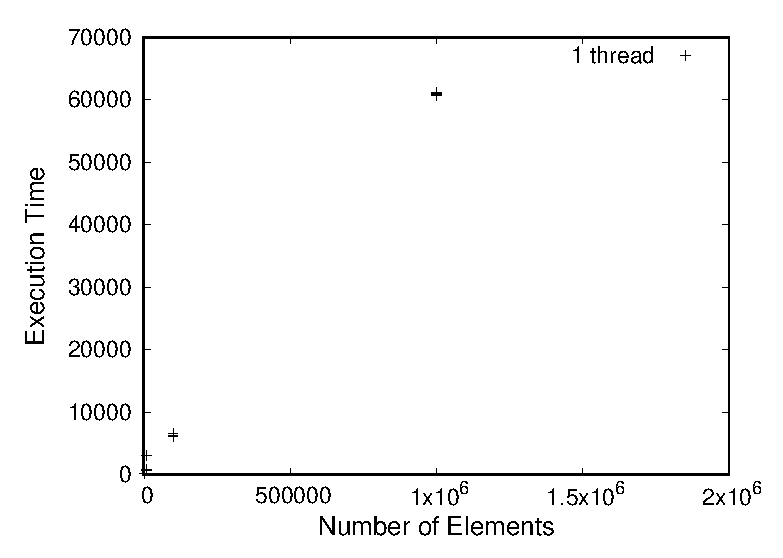
\includegraphics[width=\columnwidth]{o1.eps}
 \caption{N=1}
 \label{fig:part1}
\end{subfigure} \hfill
%
\begin{subfigure}{0.41\linewidth}
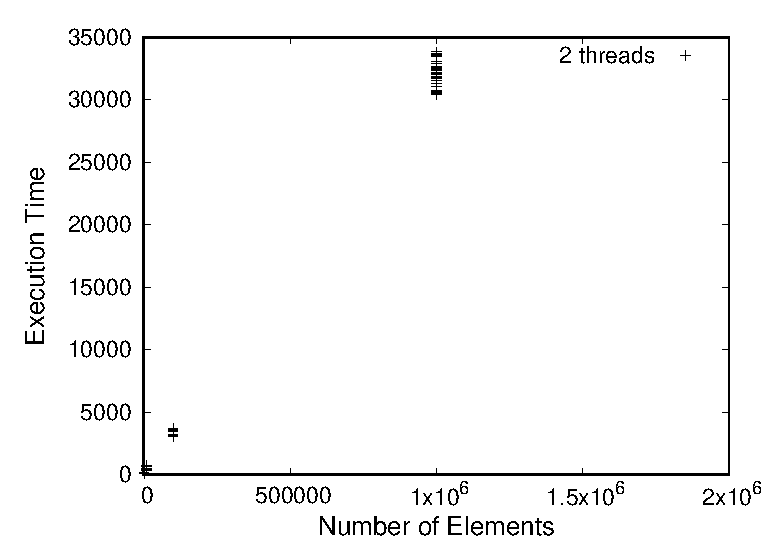
\includegraphics[width=\columnwidth]{o2.eps}
 \caption{N=2}
 \label{fig:part2}
\end{subfigure} \hfill
%

\centering
\begin{subfigure}{0.41\linewidth}
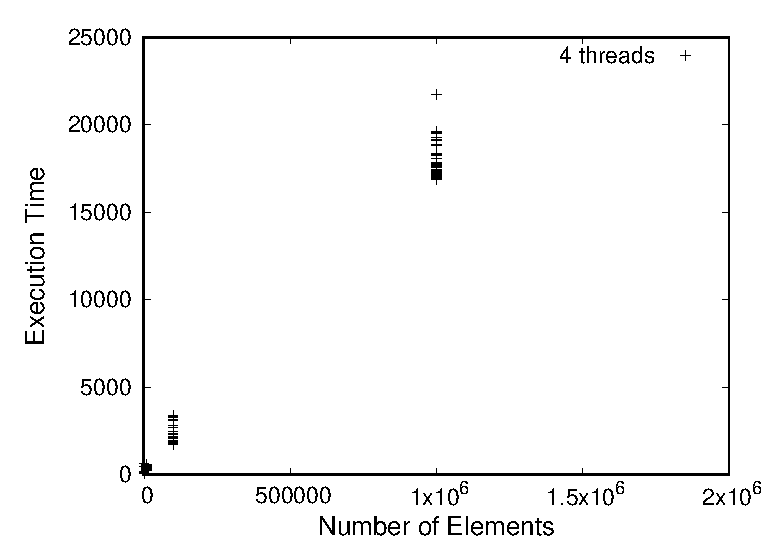
\includegraphics[width=\columnwidth]{o4.eps}
 \caption{N=4}
 \label{fig:part1}
\end{subfigure} \hfill
%
\begin{subfigure}{0.41\linewidth}
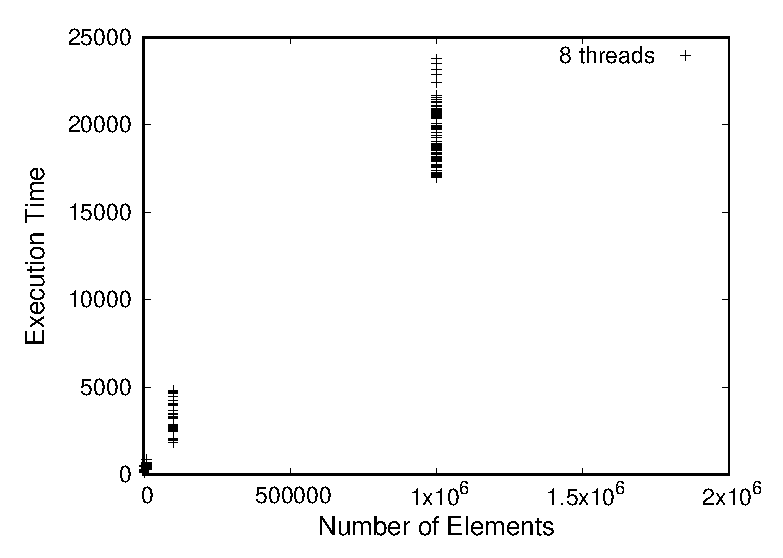
\includegraphics[width=\columnwidth]{o8.eps}
 \caption{N=8}
 \label{fig:part2}
\end{subfigure} \hfill
%
\centering
\begin{subfigure}{0.41\linewidth}
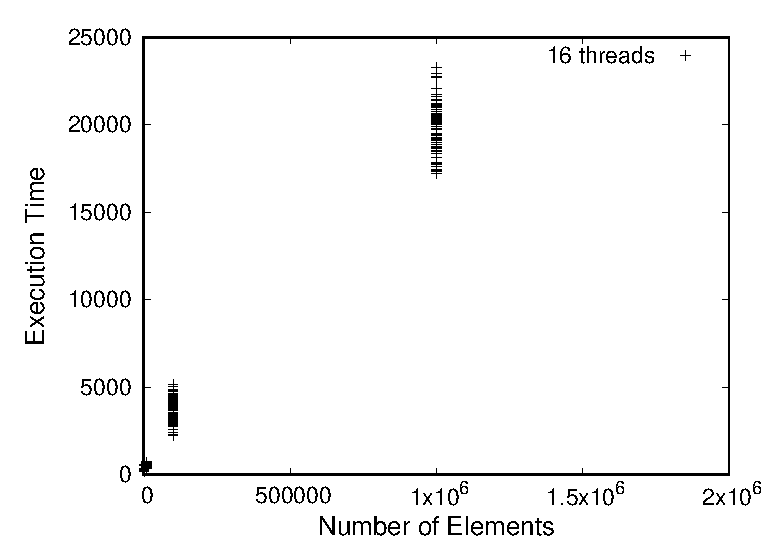
\includegraphics[width=\columnwidth]{o16.eps}
 \caption{N=16}
 \label{fig:part1}
\end{subfigure} \hfill
\caption{Scatter Plots for different values of N(=Number of threads).}
\label{fig:composite}
\end{figure}

\begin{figure}
\centering
\begin{subfigure}{0.41\linewidth}
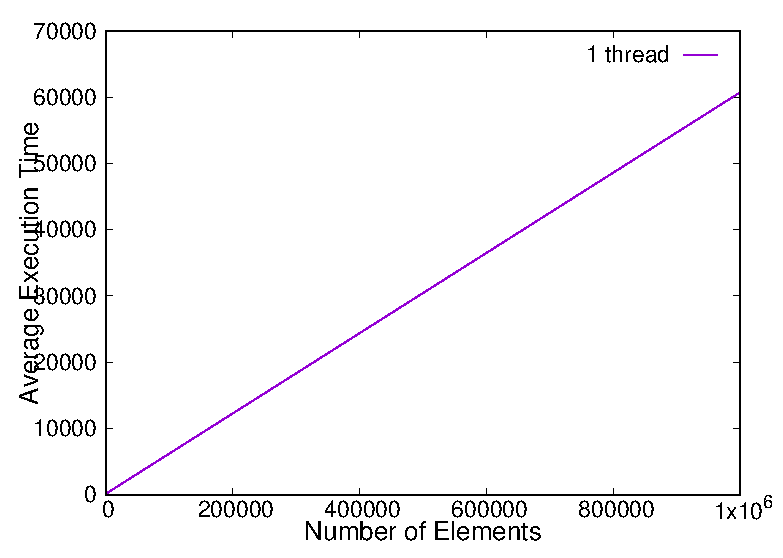
\includegraphics[width=\columnwidth]{l1.eps}
 \caption{N=1}
 \label{fig:part1}
\end{subfigure} \hfill
%
\begin{subfigure}{0.41\linewidth}
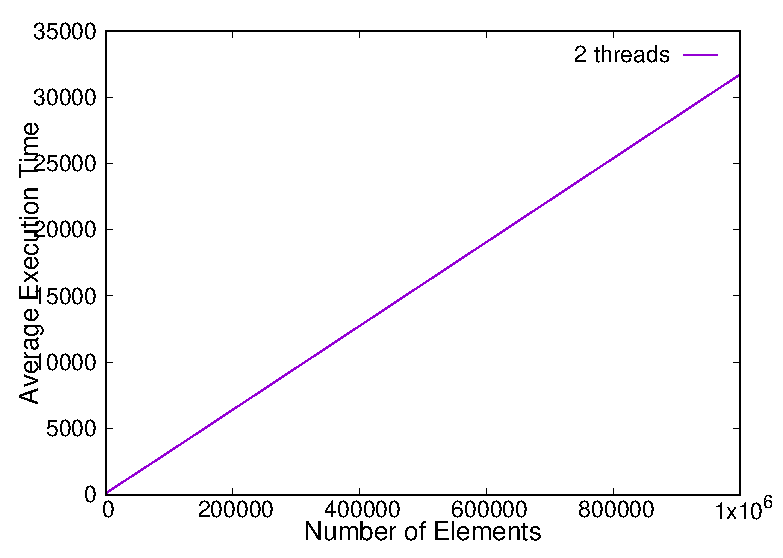
\includegraphics[width=\columnwidth]{l2.eps}
 \caption{N=2}
 \label{fig:part2}
\end{subfigure} \hfill
%

\centering
\begin{subfigure}{0.41\linewidth}
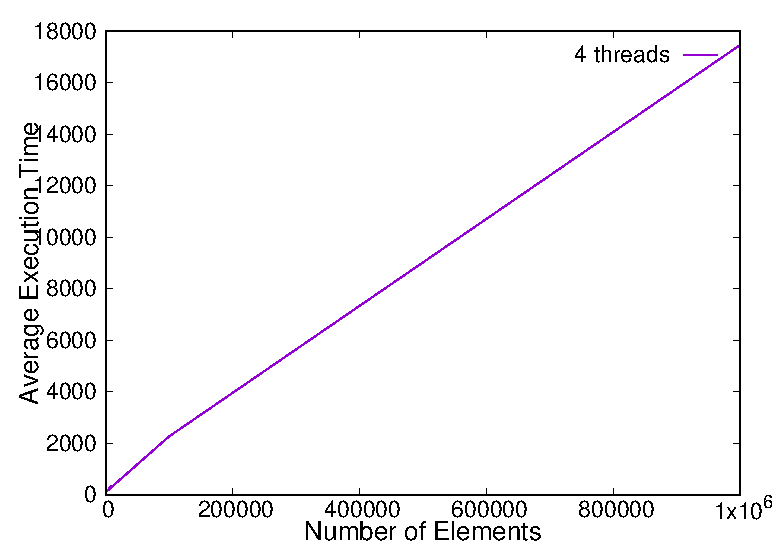
\includegraphics[width=\columnwidth]{l4.eps}
 \caption{N=4}
 \label{fig:part1}
\end{subfigure} \hfill
%
\begin{subfigure}{0.41\linewidth}
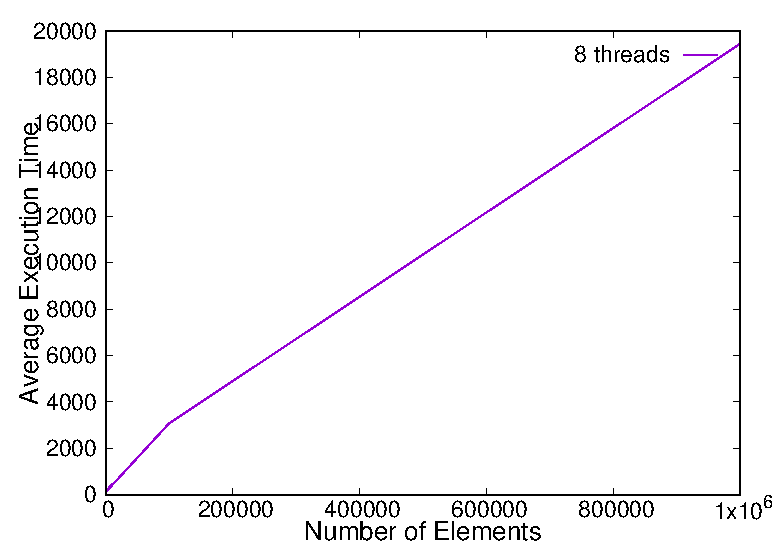
\includegraphics[width=\columnwidth]{l8.eps}
 \caption{N=8}
 \label{fig:part2}
\end{subfigure} \hfill
%
\centering
\begin{subfigure}{0.41\linewidth}
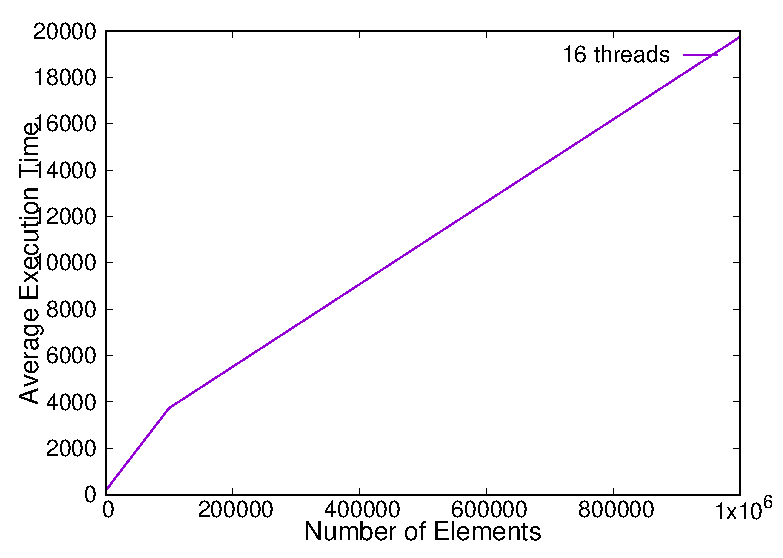
\includegraphics[width=\columnwidth]{l16.eps}
 \caption{N=16}
 \label{fig:part1}
\end{subfigure} \hfill
\caption{Line Plots for different values of N(=Number of threads).}
\label{fig:composite}
\end{figure}

\begin{figure}
\centering
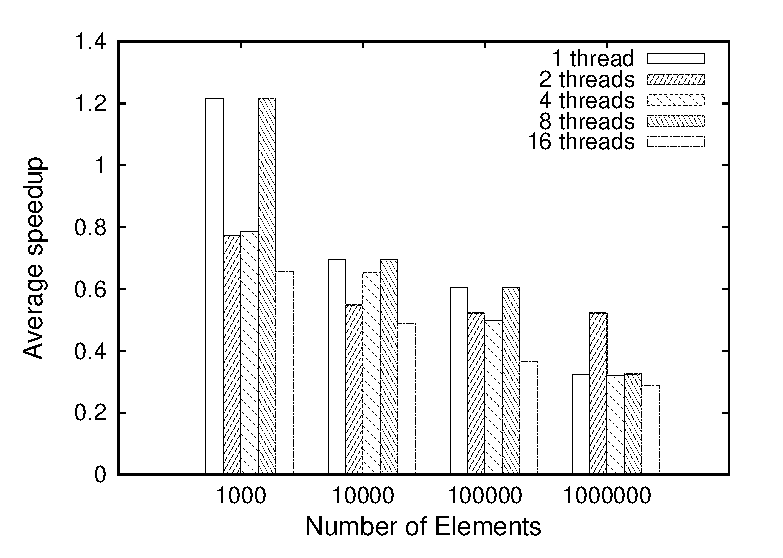
\includegraphics[width=0.7\columnwidth]{bar.eps}
 \caption{Average Speedup Bar Graph}
 \label{fig:Bar Graph for Average Speedup}
\centering
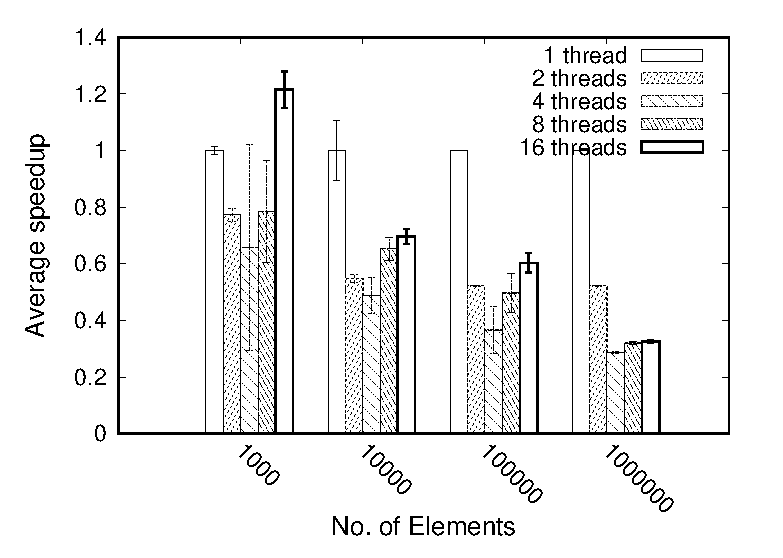
\includegraphics[width=0.7\columnwidth]{error.eps}
 \caption{Average Speedup with Error Bars}
 \label{fig:Average Speedup Bar Graph with Errors}
\end{figure}
\end{document}
